\documentclass[11pt,conference]{IEEEtran}
\IEEEoverridecommandlockouts
% The preceding line is only needed to identify funding in the first footnote. If that is unneeded, please comment it out.
\usepackage{cite}
\usepackage{amsmath,amssymb,amsfonts}
\usepackage{graphicx}
\usepackage{textcomp}
\usepackage{soul}
\usepackage{xcolor}
\usepackage[english]{babel}
\usepackage[utf8]{inputenc}
\usepackage{algorithm}
\usepackage[algo2e]{algorithm2e} 
\usepackage[noend]{algpseudocode}


\def\BibTeX{{\rm B\kern-.05em{\sc i\kern-.025em b}\kern-.08em
\kern-.1667em\lower.7ex\hbox{E}\kern-.125emX}}
\begin{document}

\title{Using Machine Learning To Solve Text-based CAPTCHAs\\
}

\author{\IEEEauthorblockN{Turhan Kimbrough}
\IEEEauthorblockA{\textit{Department of Computer Science} \\
\textit{Towson University}\\
Towson, Maryland\\
tkimbr1@students.towson.edu}
}

\maketitle

\begin{abstract}
	CAPTCHA is an acronym for the "Completely Automated Public Turing test
	to tell Computers and Humans Apart". It is a mechanism which is used to
	deter bots from abusing software systems. CAPTCHAs come in a variety of forms,
	including the deciphering of obfuscated text, transcribing of audio messages,
	tracking mouse movement, and more. This research will focus on automating the
	process of deciphering text-based CAPTCHAs using machine learning
	techniques. Specifically, supervised learning and convolutional neural
	networks are used to develop
	a model which is capable of over 99\% accuracy for certain datasets. 
	The goal of this research is to demonstrate the weaknesses associated with text-based
	CAPTCHA mechanisms, especially with the prevalence of machine learning
	tools.
\end{abstract}

\begin{IEEEkeywords}
	machine learning, neural networks, supervised training, CAPTCHA
\end{IEEEkeywords}

\section{Introduction}
CAPTCHA is an acronym for the "\textbf{C}ompletely \textbf{A}utomated
\textbf{P}ublic \textbf{T}uring test to tell
\textbf{C}omputers and \textbf{H}umans \textbf{A}part", which is a
challenge-response test used in computing services to verify that the user is a
human. The premise of a CAPTCHA is to provide a test which is relatively easy
for a human to solve, but difficult for bots. This is one of many 
mechanisms used to combat against the growing usage of malicious software
automation. Due to the ubiquity of automation software, cybercriminals have
been able to easily create bots to perform malicious acts. These acts include
denial-of-service attacks, autonomous social media communication agents,
scalping scarce merchandise, and more.

Due to the wide availability of CAPTCHA-generating software, they have become a popular
mechanism to integrate into websites. In particular, text-based CAPTCHAs are
often available as a low-cost and simple solution. Text-based CAPTCHAs
typically consist of alphanumeric characters in an image, which has been
manipulated to prevent it from being easily parsed by a machine. Users are then
challenged to decipher the text in the CAPTCHA, and if the answer is correct,
they can continue using the service. CAPTCHAs are typically available from
content management systems (such as WordPress) or can be integrated into a
website via API.

\begin{figure}[htbp]
	\centerline{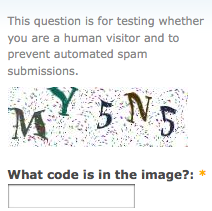
\includegraphics[scale=0.7]{images/alphanumeric-captcha.png}}
	\caption{Example of a text-based CAPTCHA.}
	\label{figure}
\end{figure}

While this mechanism can mitigate the majority of software bots, it may pose
trouble against bots utilizing machine learning technology. This research
paper demonstrates that a machine learning agent is capable of solving CAPTCHAs
with the use of open-source tools, supervised training, and convolutional
neural networks. The goal of this research is show how adversaries can use
readily available technologies to exploit text-based CAPTCHA mechanisms.
This paper will cover background/related work, the methodology  used for
solving CAPTCHAs, results, challenges, future work, and concluding thoughts.

\section{Background/Related Work}
In this section, there will be a brief review of similar work which has been
done with machine learning and CAPTCHAs.

\subsection{Solving reCAPTCHAs With Reinforcement Learning}
Researchers at \hl{[]} have demonstrated the ability to solve mouse-based reCAPTCHAs using
reinforcement learning. Google's reCAPTCHA mechanism is more difficult to solve
compared to traditional CAPTCHAs due to its usage of mouse-tracking to
determine if the user is a human. While the exact algorithm is unknown due to
the closed-source nature of the reCAPTCHA technology, the researchers use a
black-box approach to solve reCAPTCHAs.

The approach models mouse movements as transitions on a 2-dimensional grid
of pixels. The \emph{Markov Decision Process} is used to generate a series of
movements (up, down, left, right), which is combination of random and controlled
outcomes. The mouse-controlled agent is then trained through reinforcement
learning to generate a series of movements which mimic the behavior of humans.
This methodology was able to achieve a success rate of 97.4\% on a 100x100
grid and 96.7\% on a 1000x1000 display.

\begin{figure}[htbp]
	\centerline{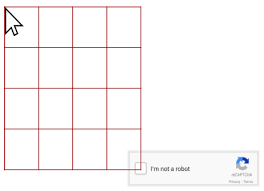
\includegraphics[scale=0.5]{images/grid-world.png}}
	\caption{Grid world model.}
	\label{figure}
\end{figure}

\subsection{Generic Solving of Text-based CAPTCHAs}
Researchers at \hl{[]} have provided a basic framework on solving CAPTCHAs using
segmentation and character recognition techniques. More specifically, their
technique is able to detect individual characters in CAPTCHAs with occluding
lines. Traditional approaches to CAPTCHA-solving typically use two separate
algorithms for segmentation and character recognition. The researchers have
instead, developed an algorithm which combines the steps of segmentation and character
recognition.

The researchers approached this solution by studying previous schemes which
were used to analyze characters in CAPTCHAs. Many of them were unable to
segment CAPTCHAs which used \emph{negative kerning}, a technique
where negative space is used between characters to ensure occlusion 
by their neighbors. The algorithm developed by the researchers use machine
learning to perform 3 steps: \emph{cut-point detection}, \emph{slicing}, and
\emph{scoring}.
Cut-point detection analyzes all combinations of character partitioning. The
slicer will then segment each character using every partitioning combination,
placing them in a graph afterwards. Finally, the scorer assigns a weight for
each partitioning combination and determines which characters are most likely
present in the CAPTCHA.

\begin{figure}[htbp]
	\centerline{
\includegraphics[scale=0.5]{images/negative-kerning.png}}
	\caption{Example of negative kerning.}
	\label{figure}
\end{figure}

\subsection{Immutable Adversarial Examples for CAPTCHA Generation}
While the two works above demonstrate the exploitation of CAPTCHAs, the work
presented here will demonstrate an approach for securing CAPTCHAs. Researchers
at \hl{[]} have demonstrated the ability to produce CAPTCHAs which are resistant to
noise-removal attempts. Often, CAPTCHA solving techniques using neural networks
apply filters to a CAPTCHA image; reducing noise and exaggerating features. Generating CAPTCHAs with immutable noise would pose a significant
challenge to many of the machine learning assisted CAPTCHA solvers.

The researchers were able to create immutable adversarial CAPTCHAs by using a
modification of the \emph{fast gradient sign} (FGS) method. The FGS method
works by slightly altering the gradient values of certain image pixels to
maximize \emph{loss} (bad predictions) during the training process of a neural network. The
modified FGS method takes a target label and confidence level as inputs in
addition to the original image. This allows for noise generation to work
towards a specific goal, distributing the noise in such a way that is
difficult to filter.

\begin{figure}[htbp]
	\centerline{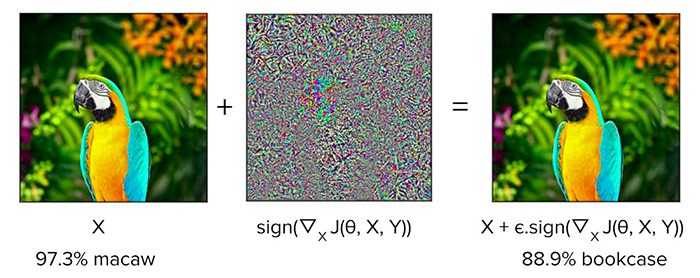
\includegraphics[scale=0.35]{images/fgsm_technique.png}}
	\caption{FGS method fooling a machine learning model.}
	\label{figure}
\end{figure}

\section{Methodology}

In this section, a proof-of-concept CAPTCHA-solving model is constructed using
open-source tools and machine learning principles. The first two subsections
will give background information on the tools/principles being applied. The
rest of the subsections will walk through the procedure for creating the machine
learning model.

\subsection{Open-source Tool Selection}
\emph{Python 3} will be the programming language of choice, due to its
easy-to-use syntax, portability, and wide range of modules. To complement
Python 3, the \emph{Python Image Library (PIL)} will be used to generate
CAPTCHA images, and \emph{TensorFlow} will be the core library for building the
machine learning model. Lastly, the code will be written for the \emph{Jupyter
Notebook} environment, a popular open-source web application for creating/sharing
documents in the scientific community.

\subsection{Applied Machine Learning Principles}
Two core machine learning principles will be applied when creating the
CAPTCHA-solving model, \emph{convolutional neural networks (CNN's)} and
\emph{supervised learning}. These two principles are commonly used for
image-processing, a perfect use-case for CAPTCHA-solving.

CNN's are a subset of \emph{artificial neural networks (ANN's)}, a family of algorithms
which mimic the structure of biological neural networks found in animal brains
\hl{[]}.
ANN's consist of an input layer for data, one or more hidden layers for
data-processing, and an output layer for decision-making. CNN's use
a combination of \emph{convolutional layers} and \emph{pooling layers} to
represent the hidden layers in its structure. Convolutional layers are used to
create feature maps, a technique used to extract characteristics from image
data \hl{[]}. A pooling layer is placed after each convolutional layer to reduce the
size of each feature map, lowering the computation power required for
further processing \hl{[]}.

Supervised learning is a technique to train a machine learning model with
the use of labelled data. The labels in the dataset define a category or
feature for each data instance \hl{[]}.

\begin{figure}[htbp]
	\centerline{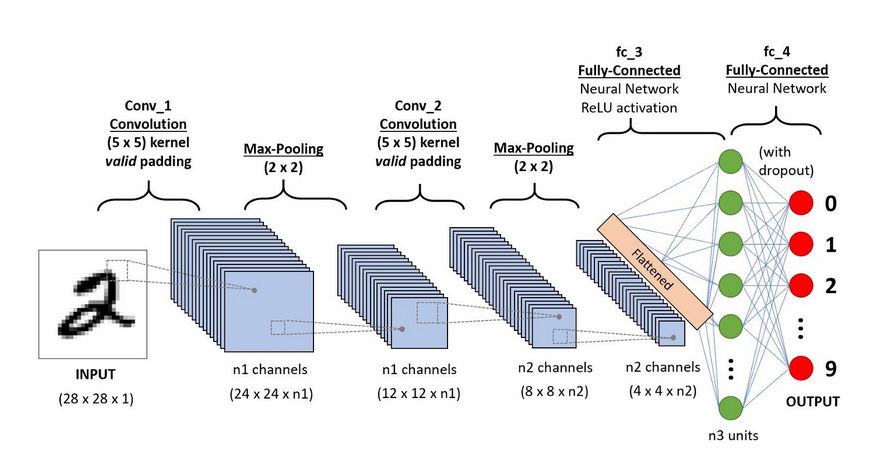
\includegraphics[scale=0.25]{images/cnn-example.png}}
	\caption{Example structure of convolutional neural network.}
	\label{figure}
\end{figure}


\subsection{Creating the Training Data}
Creating the training dataset consists of two parts; generating a large series
of CAPTCHA images and creating labels for each one. In order to
satisfy these two requirements, PIL will be used to generate CAPTCHA images
with their labels. 

In a script using PIL, a total of 10,000 images will be generated. This creates a representative
population of 4-digit CAPTCHAs ranging from '0000' to '9999'. Each image will use a dimension of 
100x100 pixels along with a consistent font \emph{(DejaVu Sans)}. To obfuscate the
text, each image will contain random colored dots and lines. A different color
will also be used to print the text in each image. Afterwards, the image will be saved
as a PNG image file, with the 4-digit string included in the file name. All
CAPTCHA images will be saved in the same directory for processing later on.

\begin{algorithm}
	\caption{Generating labelled CAPTCHAs}
		\State $count \leftarrow 0 $
		\State
		\While{$count < 10,000$} { 
		\State $number \leftarrow \Call{GetFourDigitString}{count} $
		\State $font \leftarrow \Call{GetSystemFont}{\null} $
		\State $captcha \leftarrow \Call{CreateImageWithText}{font, number} $
        \State \Call{Resize}{$captcha, 100, 100} $
        \State \Call {ColorText}{$captcha} $
		\State \Call{DrawColoredLines}{$captcha} $
		\State \Call{DrawColoredDots}{$captcha} $
		\State $captcha\_name \leftarrow number + "\_image.png" $
		\State \Call{Save}{$captcha, captcha\_name} $
		\State $count \leftarrow count + 1 $
		\EndWhile}
\end{algorithm}

\begin{figure}[htbp]
	\centerline{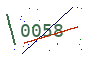
\includegraphics[scale=1.5]{images/0058_image.png}}
	\caption{0058\_image.png}
	\label{figure}
\end{figure}

The rest of the model-building procedure will take place in the \emph{Jupyter
Notebook}
file. \emph{TensorFlow} will need to be imported along with a helper library,
\emph{pandas}. The pandas library contains many data structures which are
commonly used with TensorFlow. The CAPTCHA images will need to be organized for
TensorFlow to work with, this is where the pandas \emph{DataFrame} structure
will be of use. The DataFrame is a tabular data
structure with rows denoting iterations and columns representing data
attributes.

The CAPTCHA images will be imported into the Jupyter Notebook environment,
using the directory where they were stored. A function will then
be called repeatedly to parse each file path, obtaining the 4-digit string associated with each
CAPTCHA image. The pandas DataFrame will then be used to store a pair of values
for each row; the CAPTCHA image path and its 4-digit string. This
associates the label with its respective data.


\begin{algorithm}[]
  \SetKwInOut{Input}{Input}
  \SetKwInOut{Output}{Output}
  \SetKwProg{try}{try}{:}{}
  \SetKwProg{catch}{catch}{:}{end}
  \Input{String $file\_path} 
  \Output{String $label} 

  \try{}{
    $file\_name \leftarrow \Call{SplitFileName}{file\_path} $

	\Call{SplitExtension}{$file\_name, ".png"} $

	$label \leftarrow \Call{Split}{file\_name, "\_"} $

  	\Return $label $
  }
  \catch{InvalidPathException}{
    \Return $UNSUCCESSFUL $
  }
  \caption{Get label for CAPTCHA image}
  \label{alg:exep}
\end{algorithm}

\begin{figure}[htbp]
	\centerline{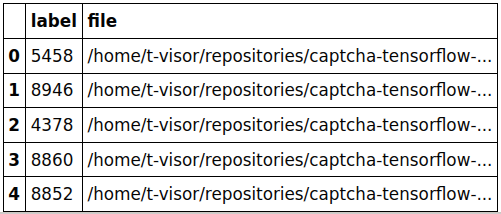
\includegraphics[scale=0.5]{images/pandas-dataframe.png}}
	\caption{Portion of resulting DataFrame.}
	\label{figure}
\end{figure}


\subsection{Defining the Neural Network Structure}
In addition to TensorFlow, the library \emph{Keras} will be used to define the
layers of the neural network. The purpose of using this neural network is to extract the features
(the sequence of digits) which are present in each CAPTCHA image.

The first layer of the neural network is the \emph{input layer}, which will be
the entry point for image data. Here, the input layer will specify each CAPTCHA image
to have a height and width of 100 pixels, and detect 3 color channels of
red, green, and blue (RGB). This will reject anomalies presented to the machine
learning model and enforce uniformity.

The \emph{hidden layers} are responsible for extracting and interpreting the
features in the image data. Through experimentation, 3
convolutional layers accompanied by 3 pooling layers have been sufficient 
for feature extraction. This set produces the optimal number of parameters (or
filters) which are required to extract the digits from each CAPTCHA image.
Afterwards, a flattening layer will transform the multi-dimensional array
representing each image into a single-dimension array for
easier processing. 2 dense layers are used afterwards for learning the features
which have been extracted from prior layers. 

The final layer of the neural network is the \emph{output layer}, which is
responsible for predicting which numbers are in a CAPTCHA image. In
particular, a reshaping layer was used to format the prediction as a
probability of numbers appearing for each digit position in the CAPTCHA.

\begin{figure}[htbp]
	\centerline{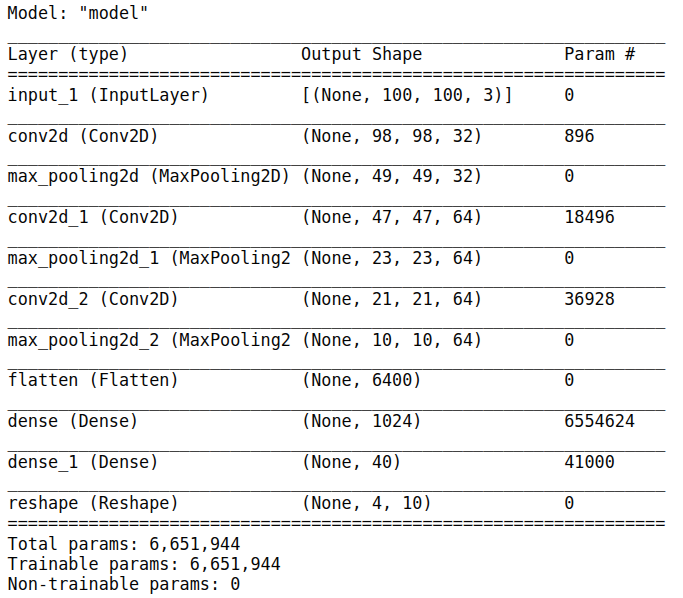
\includegraphics[scale=0.28]{images/model-summary.png}}
	\caption{Neural network layers.}
	\label{figure}
\end{figure}


\subsection{Training The Model}
Now that both the model and training data are ready for use, the training 
process may begin. There are two extra parameters which need to be defined when
the model undergoes the learning process, \emph{epochs} and \emph{batch size}.
Epochs refer to the number of training iterations while batch size
refers to the number of training samples per iteration \hl{[]}. Additionally, a batch
size can also be specified for \emph{validation}, when the model is evaluated
against a subset of the training data. 10 epochs were used
with a batch size and validation batch size of 64. These numbers were chosen as a balancing act between
training time and completeness while also avoiding \emph{overfitting}.
Overfitting is when a model memorizes the properties of 
training data to an extent that it performs negatively on new data \hl{[]}. 

\section{Results}
In this section, the metrics of the model will be analyzed along with its
performance on new data.

\subsection{Metrics}
There are two main properties to evaluate in a machine learning model, its
\emph{accuracy} and \emph{loss} over the duration of training. These two
properties share an inverse relationship; accuracy determining the model's
correctness and loss representing errors in prediction \hl{[]}. Using an additional
library, \emph{Matplotlib}, a graph representation of accuracy/loss can be
produced for the model.

\begin{figure}[htbp]
	\centerline{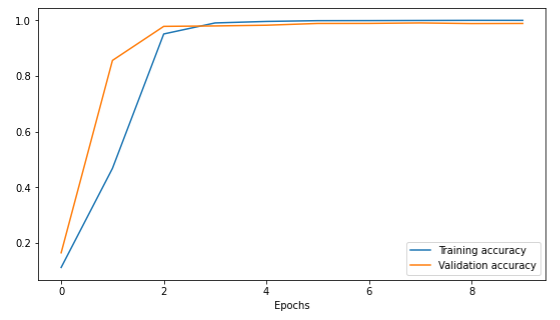
\includegraphics[scale=0.45]{images/accuracy.png}}
	\label{figure}
\end{figure}
\begin{figure}[htbp]
	\centerline{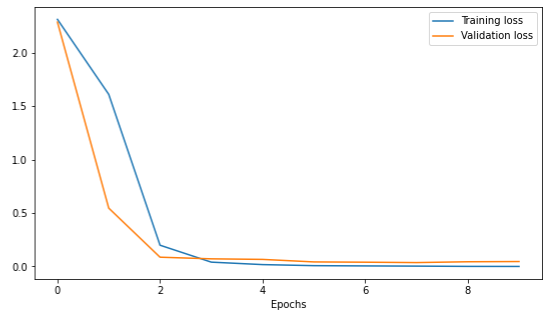
\includegraphics[scale=0.45]{images/loss.png}}
	\caption{Accuracy and loss metrics of model during training.}
	\label{figure}
\end{figure}

Accuracy is represented as a percentage, with higher percentages being favored. On
the other hand, loss is represented as a decimal value with lower values being
favored. It is important to note that a model will practically never have an
accuracy of 100\%, or a loss value of 0.

The model was able to reach over 90\% accuracy and
minimize loss to less than .5 after just 2 epochs. After 10 epochs, the model's
accuracy reached 99\% with a loss of only .03. These metrics indicate that the
model has good performance.

\subsection{Performance On New Data}
To test the performance of the model, new labelled data will need to be
generated. The same methodology for creating the training data will be used for
the \emph{test dataset}. The test dataset consists of new CAPTCHA variations
which the model has not been exposed to. The trained model will then
take each CAPTCHA image from the test dataset as input, and return a
4-digit prediction value. The \emph{Matplotlib} library will be used again to
visually represent the model's interpretation of CAPTCHA images. Each graph
instance will contain the model's prediction value, CAPTCHA image, and true
value (label for CAPTCHA image). An example of the model's performance is
demonstrated on 9 new CAPTCHA images, where it was able to accurately guess the
contents of 8 images.

\begin{figure}[htbp]
	\centerline{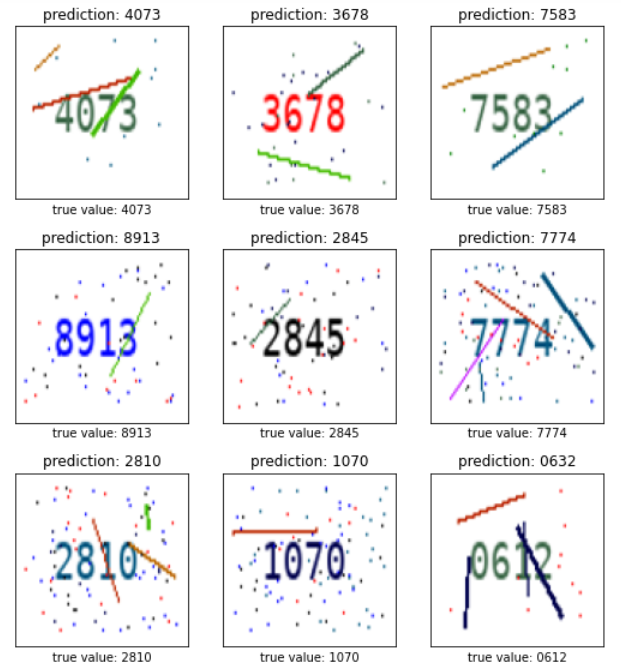
\includegraphics[scale=0.35]{images/prediction-results.png}}
	\caption{Model interpreting CAPTCHA images.}
	\label{figure}
\end{figure}

\section{Challenges}
In this section, the shortcomings of this research will be discussed.
Specifically, an adversary who uses this technique would be limited by several
factors, including the variability of CAPTCHAs and integrating the model into
automation software.

\subsection{Variability Of Real-world CAPTCHAs}
While the model produced in this research is able to accurately solve CAPTCHAs created
from the PIL library, it is unable to solve CAPTCHA images
used on live websites. This is due to the inherent variability of
CAPTCHA-generating algorithms used on different platforms. Real-world CAPTCHAs
will use a variety of fonts, image sizes, character-lengths, and distortion
techniques to produce their images. The PIL library alone would not be feasible 
for creating the variation of CAPTCHA images required for use on live websites.

\subsection{Integration Into Automation Software}
The model produced in this research is currently confined to the Jupyter
Notebook environment. For the model to be of any use to an adversary, it would
need to be exported and integrated into another software system. Currently,
TensorFlow supports model deployment to a Python application,
browser environment, web application, mobile devices, or server environment.
However, there is no general procedure for integrating the model into
browser automation software (such as Selenium). Since an adversary would want
to leverage machine learning for CAPTCHA-solving automation, creating a bot
with such capabilities is currently unfeasible.

\section{Future Work}
In this section, considerations are taken into how this research can be adapted
for future machine learning techniques.

\subsection{Multi-label Classification Technique}
One possible solution to solving a variety of CAPTCHA image styles is using 
\emph{multi-label} classification. This technique is a derivative of supervised
learning, where 2 or more labels are used for each data instance \hl{[]}. In
particular, this research can be extended by using 2 additional labels to
represent fonts and CAPTCHA string length.

\subsection{Reinforcement Learning Technique}
Another possible solution is to use \emph{reinforcement learning}. This learning technique uses a reward-based
system to incentivize certain actions over others \hl{[]}. In particular, this research
can be extended by using supervised training to recognize individual
characters and digits. Afterwards, it can be deployed to solve CAPTCHAs in a
live environment, and receive penalties/rewards based on the accuracy of its
guesses.

\subsection{Applying Principles to solve Google reCAPTCHAs}
Lastly, an interesting research direction would be to apply machine learning
techniques to solve Google's picture-based reCAPTCHAs. In particular, the
principles used in this paper, supervised learning and convolutional neural
networks, can be used for image classification. However, solving Google's picture-based
reCAPTCHAs would require insight on interpreting a photo
rather than just recognition. So in addition to using techniques in this
research, the use of reinforcement learning may provide a feasible solution.

\begin{figure}[htbp]
	\centerline{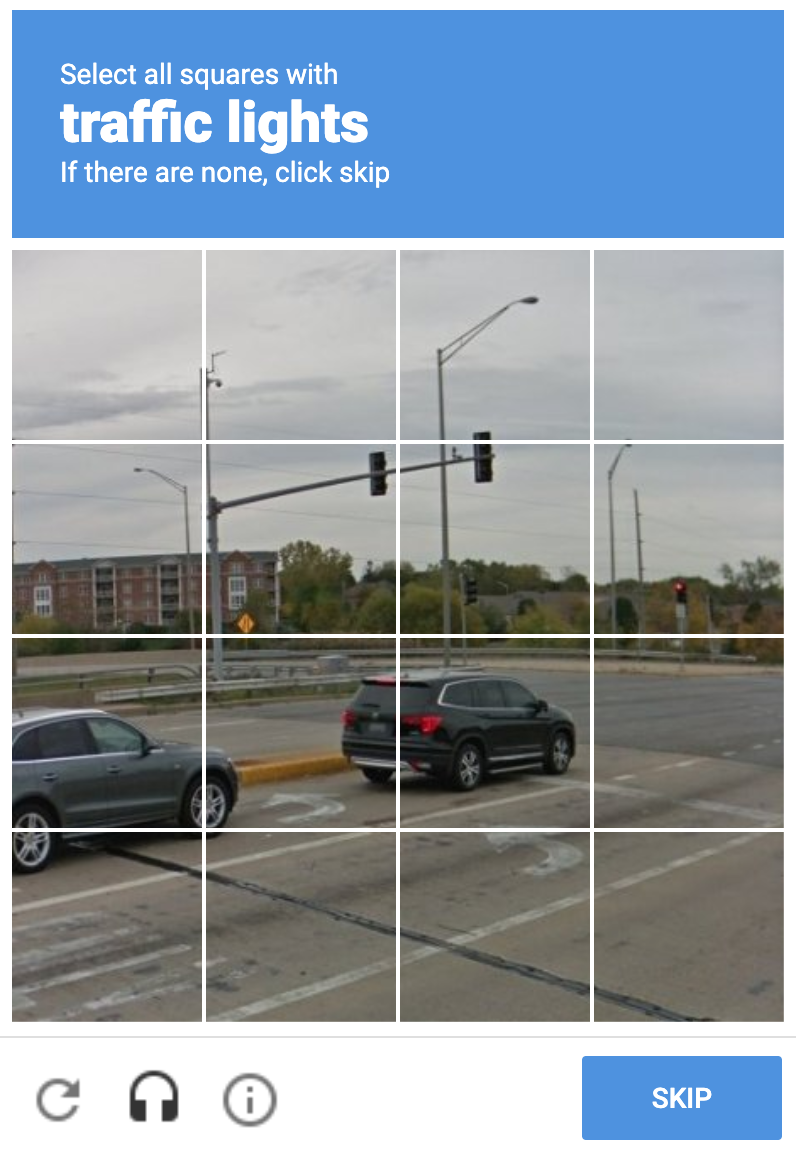
\includegraphics[scale=0.35]{images/picture-recaptcha.png}}
	\caption{Picture-based reCAPTCHA.}
	\label{figure}
\end{figure}

\section{Conclusion}
This research presents a proof-of-concept for using machine learning to assist
with CAPTCHA-solving automation. Two novel algorithms were
introduced for generating labelled CAPTCHAs and producing the corresponding
labels for the training dataset. Assuming domain knowledge on the CAPTCHAs
being solved, this work presents a simple mechanism for generating numerical variations of fixed-digit CAPTCHAs. Therefore, batches of
CAPTCHA images selected during training are representative samples. After 10
iterations of training, the resulting machine learning model had a quoted
accuracy of greater than 99\%. 

While the approach used in this research assumes access to the target's
CAPTCHA-generating algorithm, it provides a generalized framework for how
adversaries can defeat CAPTCHAs hosted on live environments. In addition,
several suggestions were provided on how this research
can be extended.

The effectiveness of the CAPTCHA-solving model in this work demonstrates the
weaknesses associated with current text-based CAPTCHA mechanisms. As machine
learning technologies evolve, so too must the defense mechanisms which are used
in current software systems.

\begin{thebibliography}{00}
	\bibitem{b1} G. Eason, B. Noble, and I. N. Sneddon, ``On certain integrals of Lipschitz-Hankel type involving products of Bessel functions,'' Phil. Trans. Roy. Soc. London, vol. A247, pp. 529--551, April 1955.
	\bibitem{b2} J. Clerk Maxwell, A Treatise on Electricity and Magnetism, 3rd ed., vol. 2. Oxford: Clarendon, 1892, pp.68--73.
	\bibitem{b3} I. S. Jacobs and C. P. Bean, ``Fine particles, thin films and exchange anisotropy,'' in Magnetism, vol. III, G. T. Rado and H. Suhl, Eds. New York: Academic, 1963, pp. 271--350.
	\bibitem{b4} K. Elissa, ``Title of paper if known,'' unpublished.
	\bibitem{b5} R. Nicole, ``Title of paper with only first word capitalized,'' J. Name Stand. Abbrev., in press.
	\bibitem{b6} Y. Yorozu, M. Hirano, K. Oka, and Y. Tagawa, ``Electron spectroscopy studies on magneto-optical media and plastic substrate interface,'' IEEE Transl. J. Magn. Japan, vol. 2, pp. 740--741, August 1987 [Digests 9th Annual Conf. Magnetics Japan, p. 301, 1982].
	\bibitem{b7} M. Young, The Technical Writer's Handbook. Mill Valley, CA: University Science, 1989.
\end{thebibliography}
\vspace{12pt}
\color{red}
IEEE conference templates contain guidance text for composing and formatting conference papers. Please ensure that all template text is removed from your conference paper prior to submission to the conference. Failure to remove the template text from your paper may result in your paper not being published.

\end{document}
